\section{Phân tích đặc trưng, nghiên cứu cắt bỏ (ablation) và quá trình hội tụ SVM}
\label{sec:thuc_nghiem_dac_trung_ablation}

\subsection{Thiết kế thí nghiệm quét lưới 729 cấu hình trên tập Validation}

Giữ lại Top-3 cấu hình tạo ứng viên đầu bảng (Lee $7\times 7, L=4$ + Otsu; Lee $7\times 7, L=1$ + Otsu; Lee $5\times 5, L=4$ + Otsu), thực nghiệm quét lưới được tiến hành:
\begin{equation}
3\text{ (lọc/ngưỡng)} \times 3\text{ (hình thái)} \times 3\text{ ($A_{\min}$)} \times 3\text{ (đặc trưng)} \times 9\text{ (mô hình)} = 729\text{ cấu hình}
\end{equation}
trên toàn bộ $671$ ảnh thuộc tập kiểm định (Validation).

\begin{figure}[!htbp]
\centering
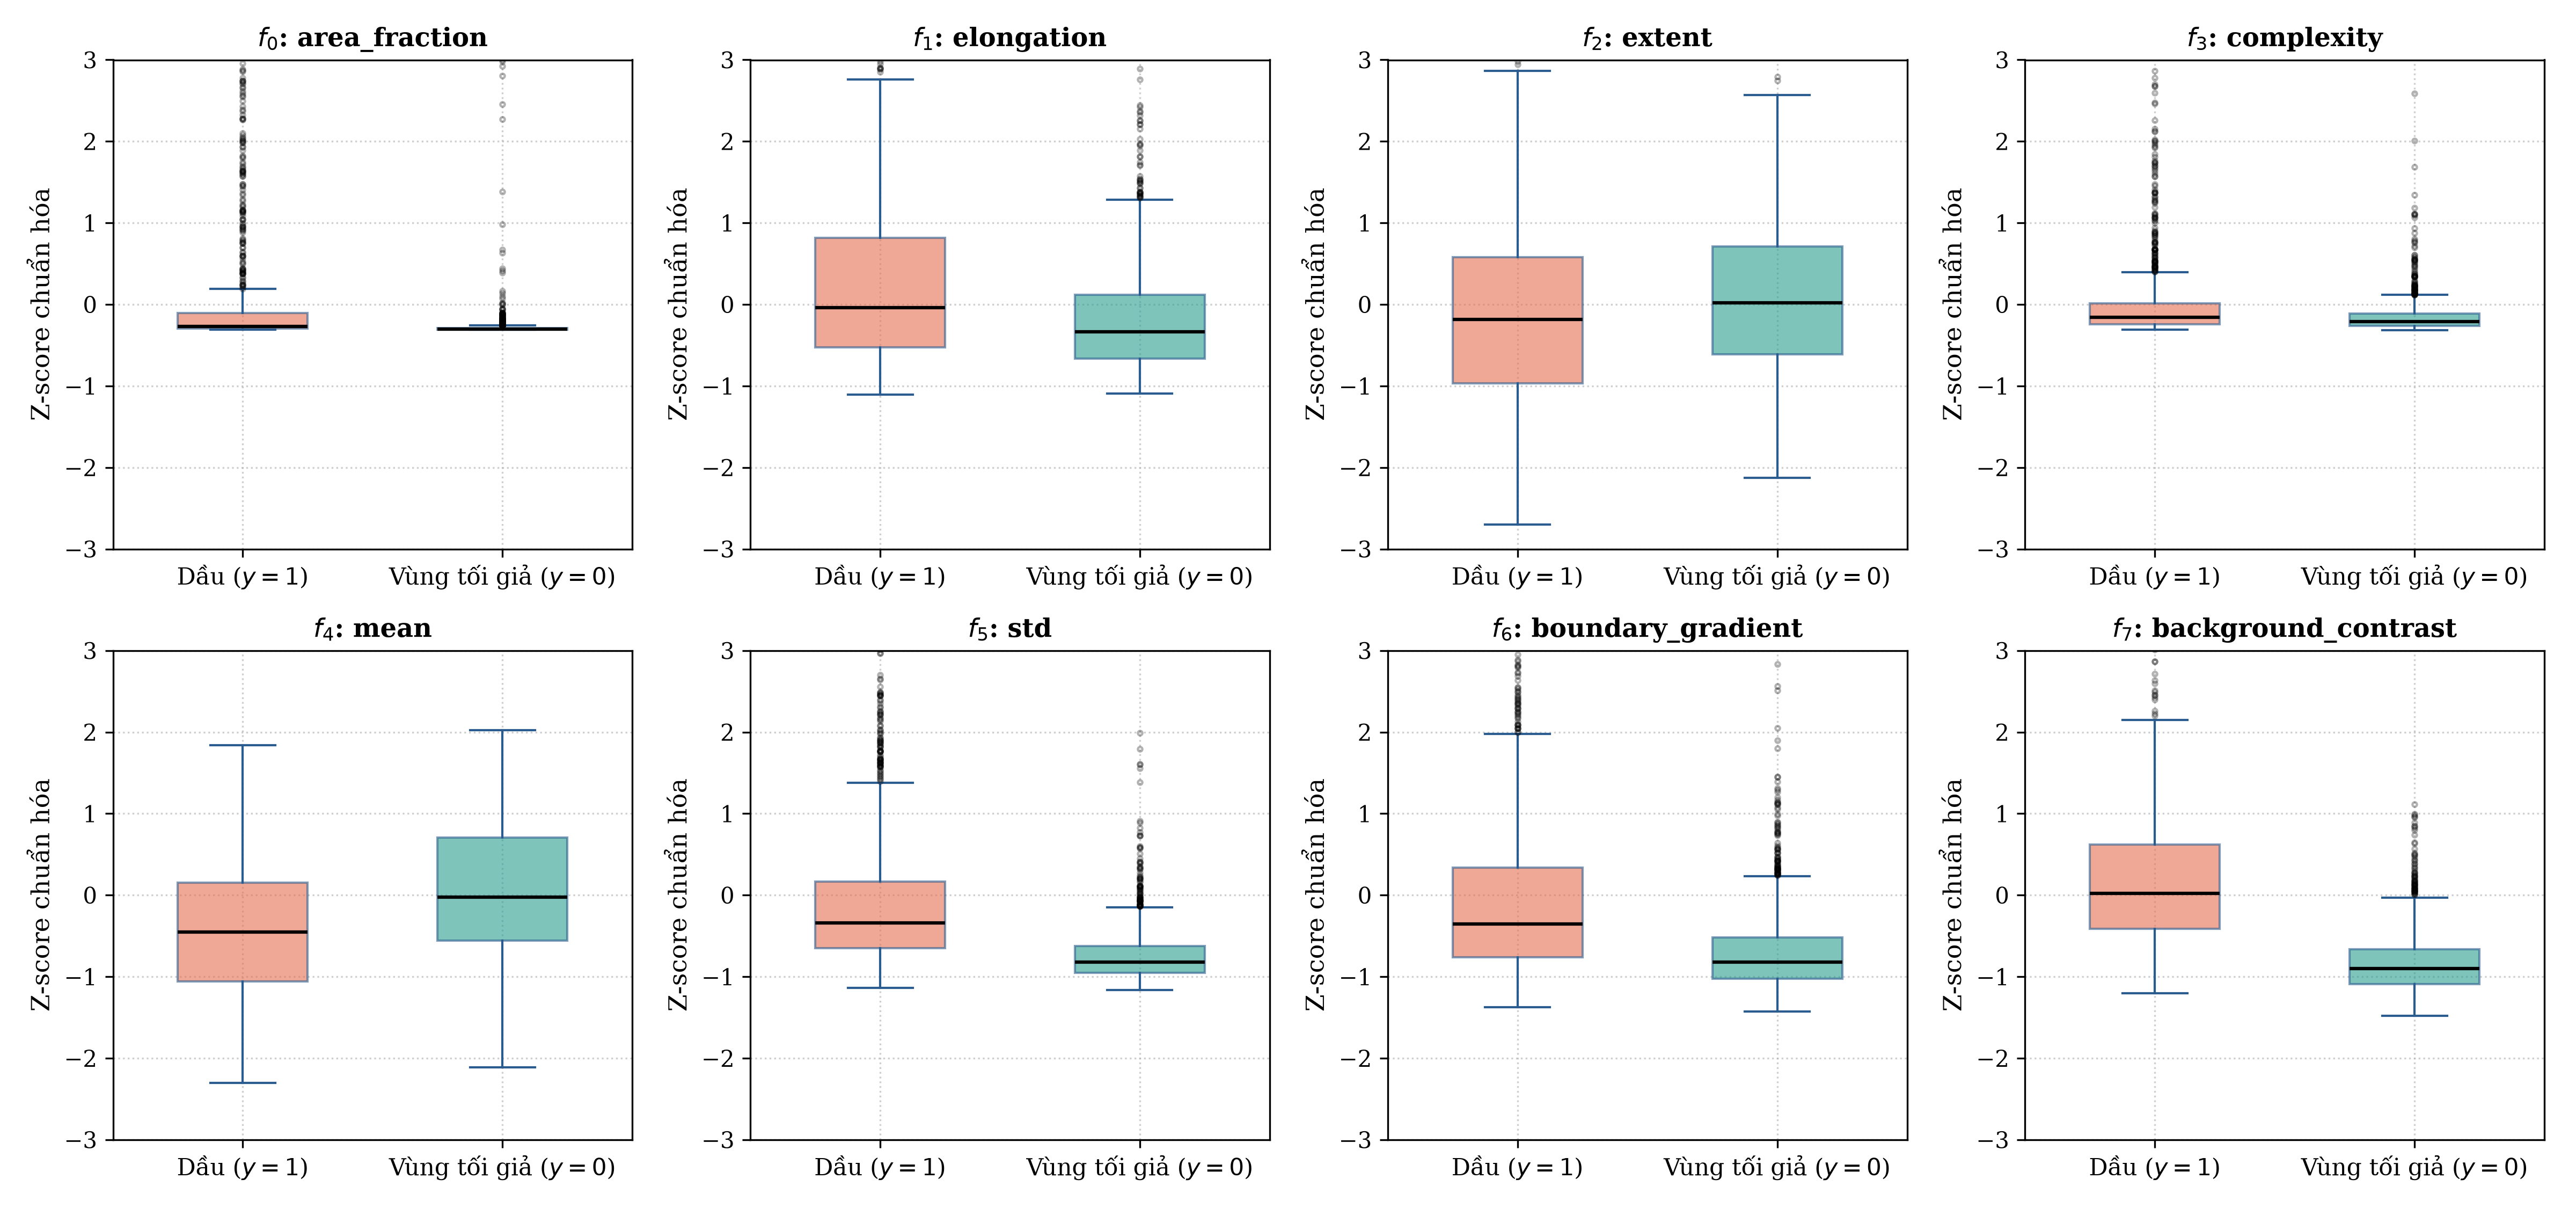
\includegraphics[width=0.98\textwidth]{figures/fig5_feature_distributions.png}
\caption{Biểu đồ Boxplot so sánh phân bố Z-score của 8 đặc trưng vùng giữa lớp Vết dầu thật ($\mathrm{Purity} \ge 0.50$, màu cam) và lớp Vùng tối báo nhầm ($\mathrm{Purity} \le 0.05$, màu xanh ngọc).}
\label{fig:feature_distributions}
\end{figure}

\begin{figure}[!htbp]
\centering
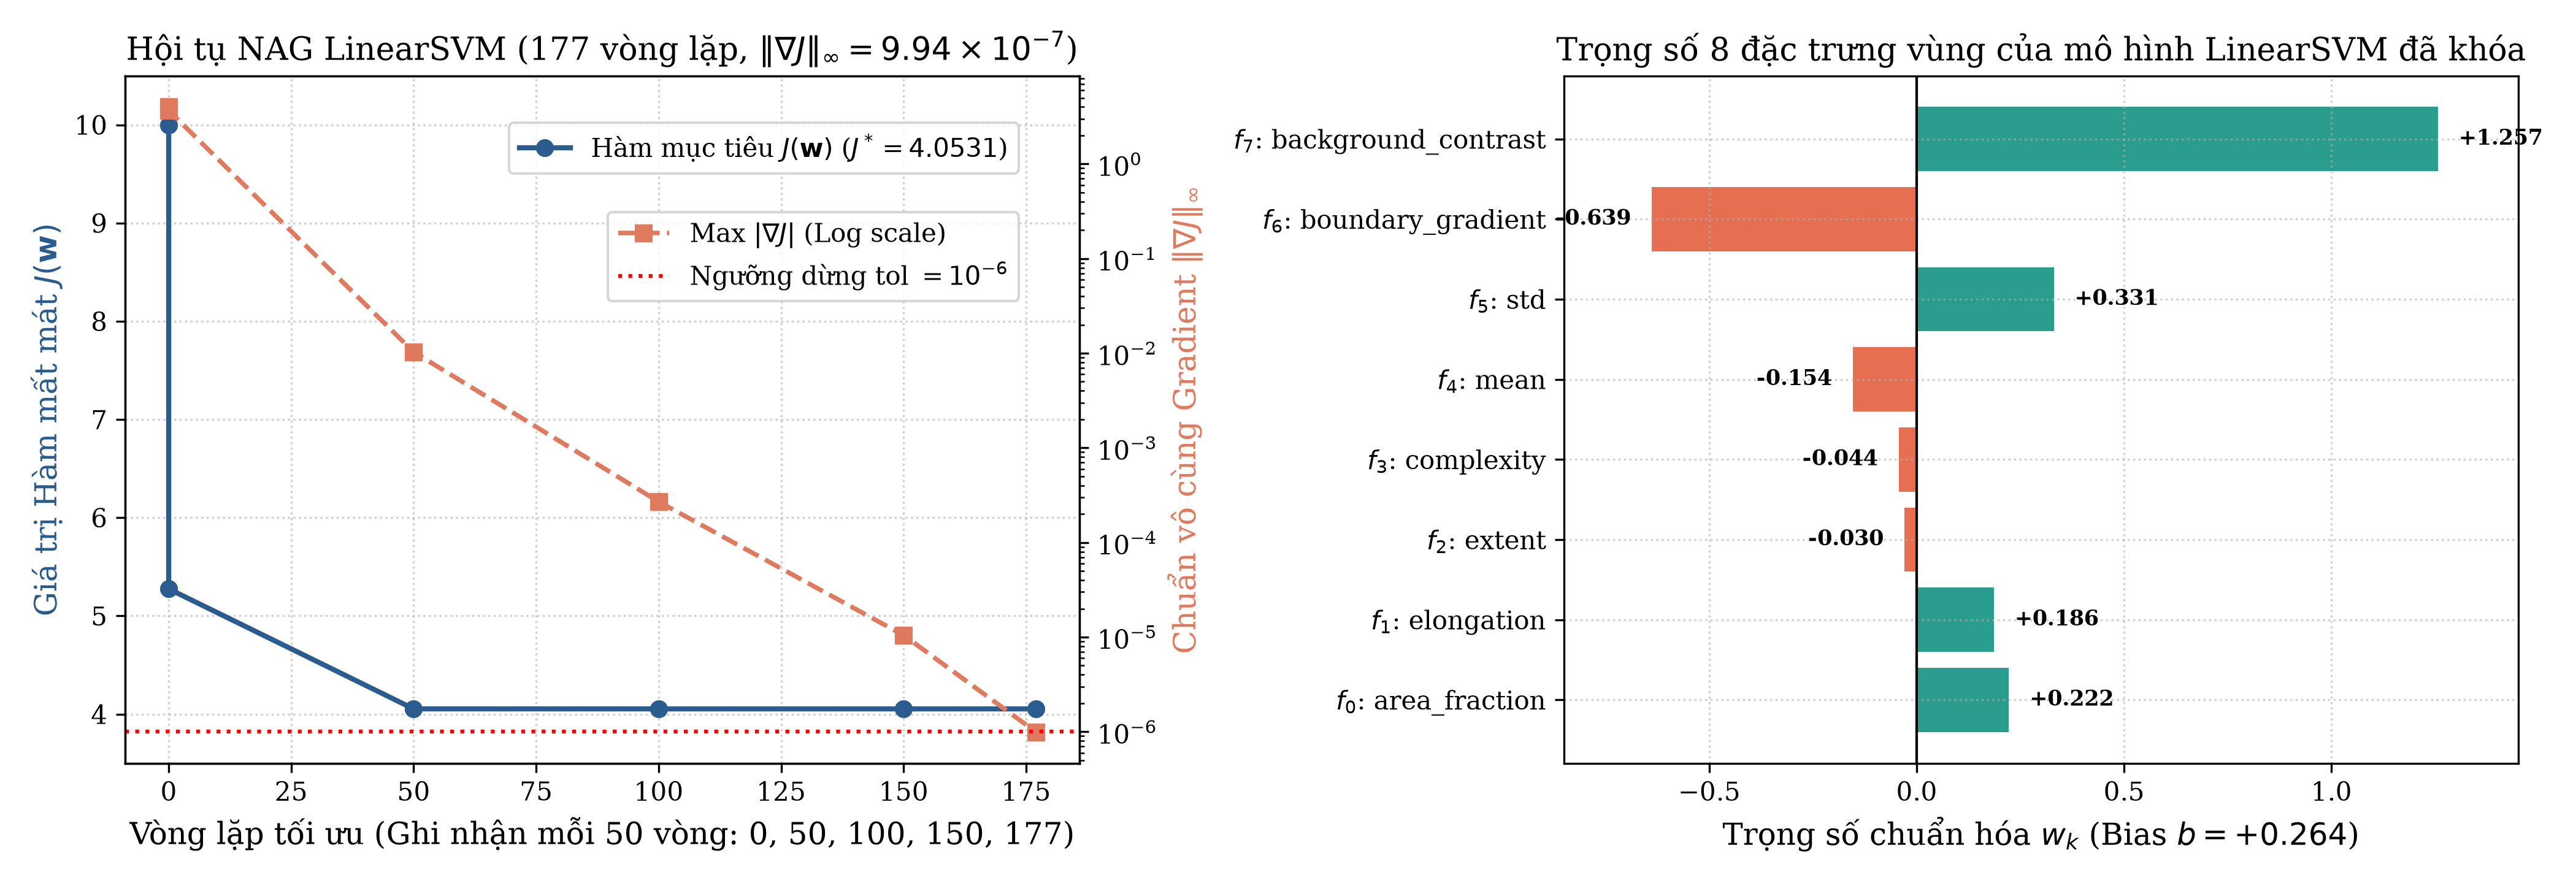
\includegraphics[width=0.96\textwidth]{figures/fig6_svm_convergence_weights.png}
\caption{Đường cong hội tụ của thuật toán tối ưu NAG và biểu đồ trọng số chuẩn hóa $w_k$ của 8 đặc trưng trong mô hình LinearSVM đã khóa.}
\label{fig:svm_convergence_weights}
\end{figure}

Bảng~\ref{tab:ablation_validation} tổng hợp kết quả của nghiên cứu cắt bỏ (Ablation study) nhằm cô lập và bóc tách tác động của từng thành phần kỹ thuật.

\begin{table}[!htbp]
\centering
\small
\caption{Kết quả khảo sát hậu xử lý, nghiên cứu cắt bỏ (Ablation) và so sánh mô hình trên 671 ảnh Validation.}
\label{tab:ablation_validation}
\resizebox{\textwidth}{!}{%
\begin{tabular}{|l|c|c|c|c|c|}
\hline
\textbf{Cấu hình khảo sát} & \textbf{TP} & \textbf{FP} & \textbf{FN} & \textbf{Object F1} & \textbf{Pixel IoU} \\ \hline
\multicolumn{6}{|l|}{\textit{1. Khảo sát ngưỡng diện tích $A_{\min}$ và hình thái học (Lee $7\times 7, L=4$ + Otsu + SVM):}} \\ \hline
$A_{\min} = 4$, \texttt{none} (Không đóng/mở) & $1\,035$ & $8\,571$ & $1\,705$ & 0.1677 & 0.6267 \\ \hline
$A_{\min} = 16$, \texttt{none} (Không đóng/mở) & $1\,034$ & $4\,482$ & $1\,706$ & 0.2505 & 0.6376 \\ \hline
$A_{\min} = 64$, \texttt{none} (\textbf{Cấu hình chọn}) & $\mathbf{1\,016}$ & $2\,215$ & $\mathbf{1\,724}$ & 0.3403 & \textbf{0.6524} \\ \hline
$A_{\min} = 64$, \texttt{close} (Đóng hình thái $3\times 3$) & 971 & $\mathbf{1\,961}$ & $1\,769$ & \textbf{0.3424} & 0.6402 \\ \hline
$A_{\min} = 64$, \texttt{open\_close} (Mở--Đóng $3\times 3$) & 988 & $2\,230$ & $1\,752$ & 0.3317 & 0.6505 \\ \hline
\multicolumn{6}{|l|}{\textit{2. Ablation theo nhóm đặc trưng (LinearSVM, $C=10, A_{\min}=64$, \texttt{none}):}} \\ \hline
Chỉ đặc trưng hình học (\texttt{shape}, 4 chiều) & 736 & $1\,737$ & $2\,004$ & 0.2824 & 0.5899 \\ \hline
Chỉ đặc trưng bức xạ/biên (\texttt{intensity}, 4 chiều) & $1\,002$ & $2\,188$ & $1\,738$ & 0.3379 & \textbf{0.6542} \\ \hline
Kết hợp toàn bộ 8 đặc trưng (\texttt{all}, đề xuất) & $\mathbf{1\,016}$ & $2\,215$ & $\mathbf{1\,724}$ & \textbf{0.3403} & 0.6524 \\ \hline
\multicolumn{6}{|l|}{\textit{3. So sánh mô hình phân loại (Nhóm đặc trưng \texttt{all}, $A_{\min}=64$, \texttt{none}):}} \\ \hline
Cây quyết định CART ($\text{depth}=3, \text{leaf}=20$) & 961 & $\mathbf{1\,998}$ & $1\,779$ & 0.3373 & 0.6456 \\ \hline
LinearSVM ($C=10$, đề xuất) & $\mathbf{1\,016}$ & $2\,215$ & $\mathbf{1\,724}$ & \textbf{0.3403} & \textbf{0.6524} \\ \hline
\multicolumn{6}{|l|}{\textit{4. Đánh giá cấp độ ứng viên theo nhãn Purity ($\mathrm{Purity} \ge 0.50$ vs. $\le 0.05$, $9\,287$ mẫu Val):}} \\ \hline
CART ($\text{TN}=6\,008$, Prec $=0.7952$, Rec $=0.7722$) & $2\,112$ & 544 & 623 & 0.7835 & -- \\ \hline
LinearSVM ($\text{TN}=5\,940$, Prec $=0.7874$, Rec $=0.8285$) & $\mathbf{2\,266}$ & 612 & $\mathbf{469}$ & \textbf{0.8074} & -- \\ \hline
\multicolumn{6}{|l|}{\textit{5. Độ nhạy theo ngưỡng nhị phân Ground Truth (LinearSVM):}} \\ \hline
Ngưỡng mặt nạ GT $M_{\text{raw}} \ge 64$ & $1\,027$ & $2\,204$ & $1\,690$ & 0.3453 & 0.6526 \\ \hline
Ngưỡng mặt nạ GT $M_{\text{raw}} \ge 128$ (Chuẩn) & $1\,016$ & $2\,215$ & $1\,724$ & 0.3403 & 0.6524 \\ \hline
Ngưỡng mặt nạ GT $M_{\text{raw}} \ge 192$ & $1\,010$ & $2\,221$ & $1\,752$ & 0.3371 & 0.6517 \\ \hline
\end{tabular}%
}
\end{table}

\subsection{Phân tích cơ chế biến ức chế và đa cộng tuyến đặc trưng}

Phân tích trọng số của mô hình LinearSVM đã khóa ($\mathbf{w} \in \mathbb{R}^8$ và bias $b = +0.264$ trên Hình~\ref{fig:svm_convergence_weights}) cho thấy cơ chế hoạt động của mô hình:
\begin{itemize}
    \item \textbf{Các đặc trưng quyết định dương tính:} Trọng số dương lớn nhất thuộc về \texttt{background\_contrast} ($w_7 = +1.257$), theo sau là \texttt{std} ($w_5 = +0.331$), \texttt{area\_fraction} ($w_0 = +0.222$) và \texttt{elongation} ($w_1 = +0.186$). Điều này khẳng định độ tương phản bức xạ giữa vùng tối và vành đai nền biển là chỉ dấu quan trọng nhất để xác nhận vết dầu loang.
    \item \textbf{Hiện tượng biến ức chế (suppressor variable) tại $w_6 = -0.639$:}
    Quan sát biểu đồ Boxplot (Hình~\ref{fig:feature_distributions}) cho thấy xét riêng lẻ từng biến (đơn biến), các vết dầu thật có trung vị độ dốc biên \texttt{boundary\_gradient} ($f_6$) cao hơn vùng tối giả, với hệ số tương quan dương $\mathrm{Corr}(f_6, y) = +0.3632$. Tuy nhiên, trong mô hình tuyến tính đa biến, $f_6$ lại nhận trọng số âm $w_6 = -0.639$.
    
    \textit{Nguyên nhân toán học:} Phân tích ma trận tương quan cho thấy $f_6$ có tương quan thuận mạnh với cả độ lệch chuẩn nội vùng $\mathrm{Corr}(f_6, f_5) = +0.8504$ lẫn độ tương phản nền $\mathrm{Corr}(f_6, f_7) = +0.6716$. Khi mô hình đã gán trọng số dương lớn cho $w_7 = +1.257$ và $w_5 = +0.331$, đặc trưng $f_6$ đóng vai trò là một \textit{biến ức chế}: trọng số âm $w_6 = -0.639$ giúp khử phần phương sai nhiễu dư thừa của các vùng có đạo hàm biên gắt do cắt ngưỡng hoặc nhiễu cục bộ nhưng lại thiếu sự chênh lệch mức xám nền tương xứng.
\end{itemize}
